\documentclass[12pt,letterpaper]{exam}
\usepackage[lmargin=1in,rmargin=1in,tmargin=1in,bmargin=1in]{geometry}
\usepackage{../style/exams}

% -------------------
% Course & Exam Information
% -------------------
\newcommand{\course}{MAT 101: Exam 3}
\newcommand{\term}{Summer -- 2022}
\newcommand{\examdate}{06/09/2022}
\newcommand{\timelimit}{85 Minutes}

\setbool{hideans}{true} % Student: True; Instructor: False

% -------------------
% Content
% -------------------
\begin{document}

\examtitle
\instructions{Write your name on the appropriate line on the exam cover sheet. This exam contains \numpages\ pages (including this cover page) and \numquestions\ questions. Check that you have every page of the exam. Answer the questions in the spaces provided on the question sheets. Be sure to answer every part of each question and show all your work.} 
\scores
%\bottomline
\newpage

% ---------
% Questions
% ---------
\begin{questions}

% Question 1
\newpage
\question[10] Plot the quadratic function $y= 6 - 4 \left( x + \dfrac{9}{2} \right)^2$ as accurately as possible. Your sketch should include the vertex and axis of symmetry. 
	\[
	\fbox{
	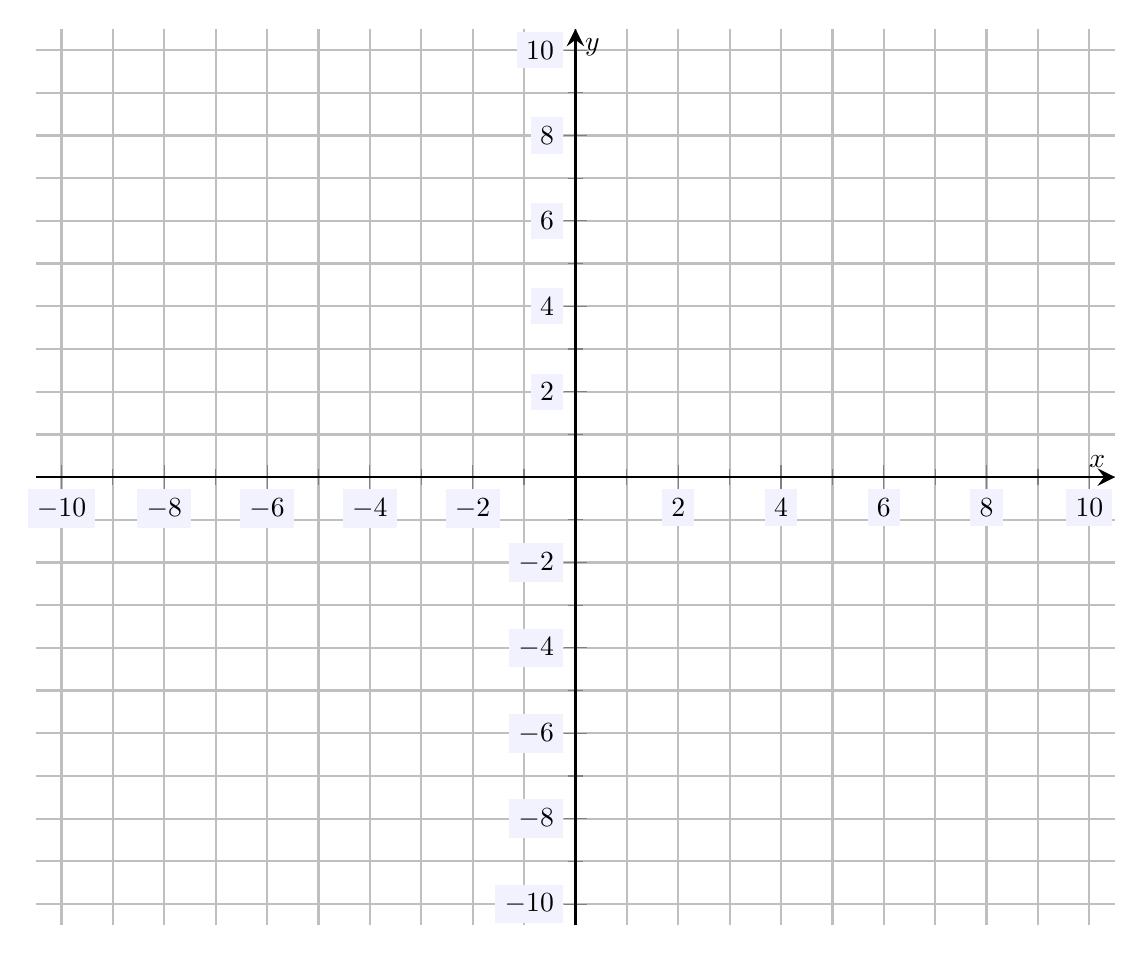
\begin{tikzpicture}[scale=2,every node/.style={scale=0.5}]
	\begin{axis}[
	grid=both,
	axis lines=middle,
	ticklabel style={fill=blue!5!white},
	xmin= -10.5, xmax=10.5,
	ymin= -10.5, ymax=10.5,
	xtick={-10,-8,-6,-4,-2,0,2,4,6,8,10},
	ytick={-10,-8,-6,-4,-2,0,2,4,6,8,10},
	minor tick = {-10,-9,...,10},
	xlabel=\(x\),ylabel=\(y\),
	]
	\end{axis}
	\end{tikzpicture}
	}
	\] 



% Question 2
\newpage
\question[10] Consider the quadratic function $f(x)= 4 - 8x - x^2$.
        \begin{enumerate}[(a)]
        \item Determine if the parabola opens upwards or downwards.
        \item Is the parabola convex or concave?
        \item Does the parabola have a maximum or minimum? 
        \item Find the vertex and axis of symmetry. 
        \item Find the maximum/minimum value of $h(x)$. 
        \end{enumerate}



% Question 3
\newpage
\question[10] Showing all your work, factor the following completely:
	\begin{enumerate}[(a)]
	\item $5x^2 - 10x$
	\item $81 - 4x^2$
	\item $x^2 - 8x - 20$
	\end{enumerate}



% Question 4
\newpage
\question[10] Showing all your work, factor the following completely:
	\begin{enumerate}[(a)]
	\item $2x^2 + 32x - 160$
	\item $10x^2 - 29x - 21$
	\end{enumerate}



% Question 5
\newpage
\question[10] Use the quadratic equation to factor the following polynomial: 
	\[
	2520x^2 + 12171x - 31680
	\]



% Question 6
\newpage
\question[10] Showing all your work and simplifying completely, solve the following:
	\[
	x^2= 3(2x - 3)
	\]



% Question 7
\newpage
\question[10] Showing all your work and simplifying completely, solve the following:
	\[
	x(x + 4)= 45
	\]



% Question 8
\newpage
\question[10] Showing all your work and simplifying completely, use the quadratic formula to solve the following:
	\[
	-8x= 10 - 8x^2
	\]



% Question 9 
\newpage
\question[10] Showing all your work and simplifying completely, use the quadratic formula to solve the following:
	\[
	\dfrac{x^2 - 14x}{3}= 159 
	\]



% Question 10
\newpage
\question[10] Showing all your work and simplifying completely, solve the following:
	\[
	\dfrac{2x - 1}{x + 5}= x - 5
	\]



% Question 11
\newpage
\question[10] Consider the following rational function:
	\[
	f(x)= \dfrac{x^2 - 4x - 5}{x^2 - 7x + 10}
	\]
Find the domain of $f(x)$. Also, find any vertical asymptotes and holes for $f(x)$. 



% Question 12
\newpage
\question[10] Showing all your work and simplifying as much as possible, compute the following:
	\[
	\dfrac{x - 7}{x^2 - 16} - \dfrac{x^2}{x^2 + 10x + 24}
	\]



% Question 13
\newpage
\question[10] Showing all your work and simplifying as much as possible, compute the following:
	\[
	\dfrac{x}{x - 1} - \dfrac{2x + 1}{x + 1} + \dfrac{6}{x}
	\]



% Question 14
\newpage
\question[10] Showing all your work and simplifying as much as possible, compute the following:
	\[
	\dfrac{x^3 - x^2}{x^2 + 3x - 40} \cdot \dfrac{x^2 + x - 30}{4x - x^2}
	\]



% Question 15
\newpage
\question[10] Showing all your work and simplifying as much as possible, compute the following:
	\[
	\dfrac{\;\;\dfrac{x^2 + 3x + 2}{24x^2 - 4x}\;\;}{\;\;\dfrac{x^2 + 14x + 24}{2x - 2x^2}\;\;}
	\]



% Question 16
\newpage
\question[10] Find all the solutions to the system of equations given by the three curves below:
	\[
	\fbox{
	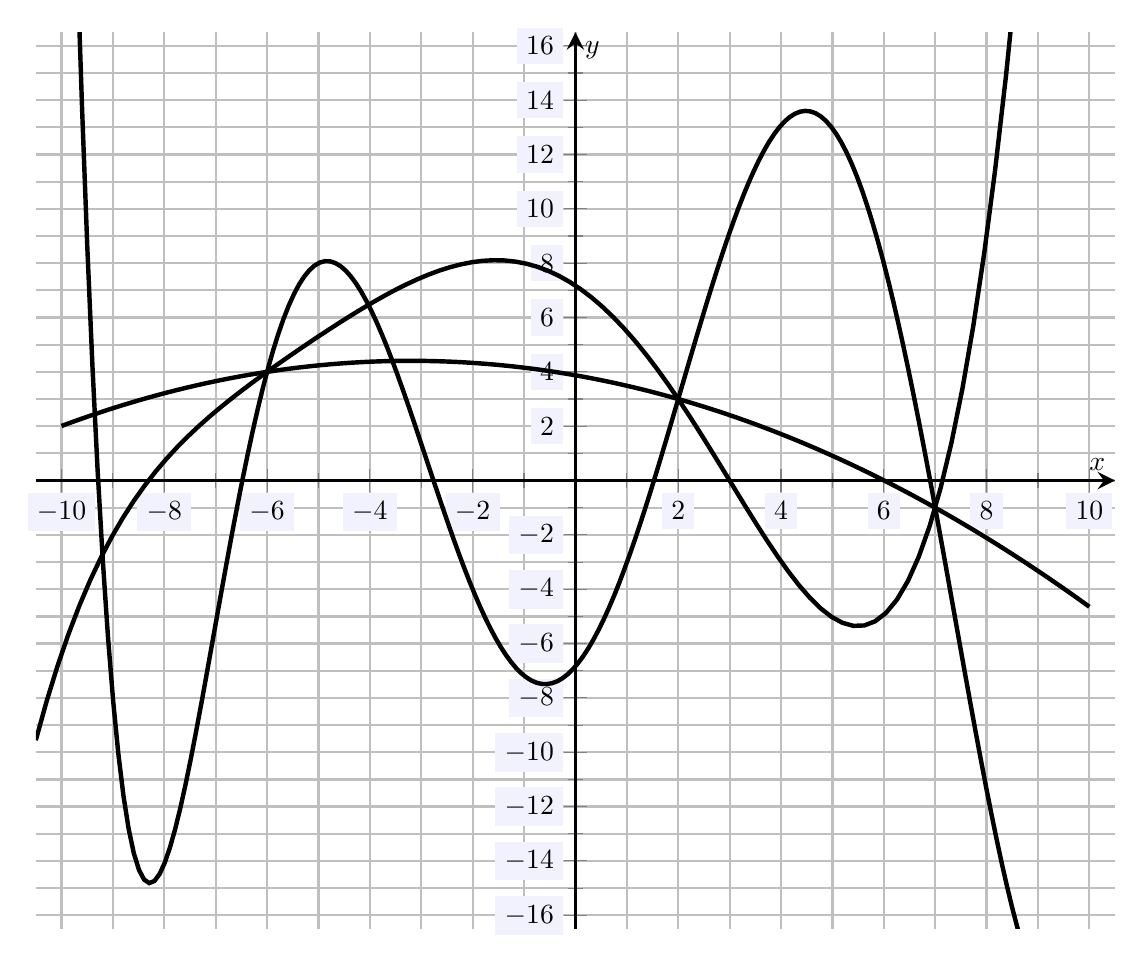
\begin{tikzpicture}[scale=2,every node/.style={scale=0.5}]
	\begin{axis}[
	grid=both,
	axis lines=middle,
	ticklabel style={fill=blue!5!white},
	xmin= -10.5, xmax=10.5,
	ymin= -16.5, ymax=16.5,
	xtick={-10,-8,-6,-4,-2,0,2,4,6,8,10},
	ytick={-16,-14,-12,-10,-8,-6,-4,-2,0,2,4,6,8,10,12,14,16},
	minor tick = {-16,-15,...,16},
	xlabel=\(x\),ylabel=\(y\),
	]
	\addplot[thick, domain= -10.5:10.5, samples=100] ({x},{0.000484337*x^5 + 0.00629318*x^4 - 0.0032989*x^3 - 0.439026*x^2 - 1.25454*x + 7.17538});
	\addplot[thick, domain= -10:10, samples=200] ({x},{-0.0000195832*x^7 + 0.000372304*x^6 + 0.00267784*x^5 - 0.0532614*x^4 - 0.122871*x^3 + 1.79151*x^2 + 2.19989*x - 6.83767});
	\addplot[thick, domain= -10:10, samples=100] ({x},{-0.0519231*x^2 - 0.332692*x + 3.87308});
	\end{axis}
	\end{tikzpicture}
	}
	\] 



% Question 17
\newpage
\question[10] Fully justifying your answer, determine if the following system of equations has a solution:
	\[
	\begin{cases}
	x + 3y= 6 \\[0.3cm]
	-2x - 6y= 24
	\end{cases}
	\]



% Question 18
\newpage
\question[10] Fully justifying your answer, determine if $(-2, 7)$ is a solution to the following system of equations:
	\[
	\begin{aligned}
	8x + 5y&= 19 \\[0.3cm]
	x + y&= 5
	\end{aligned}
	\]



% Question 19
\newpage
\question[10] Showing all your work, solve the following system of equations:
	\[
	\begin{cases}
	2x - 5y&= 1 \\[0.3cm]
	3x + 4y&= -1
	\end{cases}
	\]	



% Question 20
\newpage
\question[10] Showing all your work, solve the following system of equations:
	\[
	\begin{aligned}
	\dfrac{1}{2}\,x - y&= 7 \\[0.3cm]
	-x + \dfrac{1}{4}\,y&= -7
	\end{aligned}
	\]	


\end{questions}
\end{document}